\documentclass[10pt, twocolumn]{IEEEtran}

% Packages
\usepackage{bm}
\usepackage{url}
\usepackage{bbm}
\usepackage{cite}
\usepackage{tabu}
\usepackage{array}
\usepackage{hhline}
\usepackage{ifthen}
\usepackage{xspace}
\usepackage{dsfont}
\usepackage{balance}
\usepackage{siunitx}
\usepackage{amsmath}
\usepackage{amssymb}
\usepackage{caption}
\usepackage{graphicx}
\usepackage{multicol}
\usepackage{amsfonts}
\usepackage{mathrsfs}
\usepackage{booktabs}
\usepackage{setspace}
\usepackage{hyperref}
\usepackage{makecell}
\usepackage{footnote}
\usepackage{verbatim}
\usepackage{algorithm}
\usepackage{subcaption}
\usepackage{glossaries}
\usepackage{soul, xcolor}
\usepackage[T1]{fontenc}
\usepackage{algpseudocode}
\usepackage{algcompatible}
\usepackage[normalem]{ulem}
\usepackage{multirow, enumitem}

% Setting up packages
\captionsetup{font=footnotesize}
\setlength{\textfloatsep}{1.5pt}
\sisetup{detect-all, range-phrase=--, range-units=single, group-separator={,}}

% Initializing new commands
\newcommand{\sst}[1]{\st{#1}}
\newcommand{\tot}{\mathrm{tot}}
\newcommand{\tfrm}{T_{\mathrm{fr}}}
\newcommand{\beam}[1]{\mathcal B_{#1}}
\newcommand{\add}[1]{\textcolor{red}{#1}}
\newcommand{\size}[1]{\left | #1 \right|}
\newcommand{\bk}[1]{\textcolor{blue}{[BK: #1]}}
\newcommand{\nm}[1]{\textcolor{magenta}{[NM: #1]}}
\newcommand{\beambs}[1]{\mathcal B_{{\mathrm t},#1}}
\newcommand{\beamue}[1]{\mathcal B_{{\mathrm r},#1}}
\newcommand{\diag}[1]{\mathrm{diag}\left(#1 \right)}
\newcommand{\numberthis}{\addtocounter{equation}{1}\tag{\theequation}}
\newcommand\mst[2][red]{\setbox0=\hbox{$#2$}\rlap{\raisebox{.45\ht0}{\textcolor{#1}{\rule{\wd0}{2pt}}}}#2}

% Declaring math operators
\DeclareMathOperator*{\argmax}{arg\,max}
\DeclareMathOperator*{\argmin}{arg\,min}

% Initializing additional commands
\newcommand{\abs}[1]{\left\lvert#1\right\rvert}
\newcommand{\morn}[1]{\bigg\lVert#1\bigg\rVert}
\newcommand{\norm}[1]{\left\lVert#1\right\rVert}
\newcommand{\suchthat}{\;\ifnum\currentgrouptype=16 \middle\fi|\;}

% Redefining commands
\renewcommand\theadalign{c}
\renewcommand{\tabcolsep}{12pt}
\renewcommand\theadfont{\bfseries}
\renewcommand\cellgape{\Gape[2pt]}
\renewcommand\theadgape{\Gape[2pt]}

% Title, Authors, and Affiliations
\title{Prioritized Data Harvesting by MIMO UAVs:\\ A Multiple Traveling Salesman Problem Approach}
\author{Bharath Keshavamurthy~\IEEEmembership{Student Member, IEEE} and Nicol\`{o} Michelusi~\IEEEmembership{Senior Member, IEEE}
\thanks{The source code for this project is available on \href{https://github.com/bharathkeshavamurthy/ACCUSTOM.git}{GitHub}~\cite{Source_Code}.}
\thanks{This work has been supported by NSF under grant CNS-2129015.}
\thanks{The authors are with Electrical, Computer and Energy Engineering,}
\thanks{Arizona State University. Email: \{bkeshav1, nicolo.michelusi\}@asu.edu.}
\vspace{-12mm}}

% Content begins
\begin{document}
\bstctlcite{IEEEexample:BSTcontrol}

\maketitle
\thispagestyle{empty}
\pagestyle{empty}
\setulcolor{red}
\setul{red}{2pt}
\setstcolor{red}
\vspace{-12mm}

%%% Abstract
%% Comments:
% 1. ZF receivers at the UAVs are inverting the channel to cancel out the interference (it is not necessarily the precoding & combining design). 
%    So, rewrite the communication model technique description as "beam-forming design for MU-MIMO with spatial multiplexing (multiple spatial streams, one per user Tx antenna)".
% 2. The mTSP solution algorithm is actually called "branch-and-bound" (not "branch-and-cut"), proposed by Gavish and Srikanth.
%    Paper: [https://www.jstor.org/stable/170727]. Reference Code: [https://github.com/wasinski/VRP/blob/master/code/branchnbound.py].
%    Impl via Google OR-Tools API: [https://github.com/bharathkeshavamurthy/ACCUSTOM/blob/master/src/CrossLayerMTSPEvaluations.py].
% 3. The correct name of the trajectory design algorithm is just "Learning Competitive Swarm Optimization" (not "Learning-based Competitive Swarm Optimization").
%    Reference: [https://www.mdpi.com/1099-4300/24/2/283].
% 4. Also, I think we need to flip the solution sequence order: LCSO gives us the trajectories (and their costs) of the edges between nodes; then, mTSP branch-and-bound solves for the scheduling/association.
\begin{abstract}
This paper describes the orchestration of a fleet of MIMO-capable rotary-wing UAVs for harvesting prioritized data traffic from a random distribution of heterogeneous ground users (with MIMO capabilities). Under a finite-horizon offline formulation, the objective of this paper is to optimize the design of the precoding and combining matrices, the $3$D UAV positioning and trajectory solutions, and the user association/scheduling mechanism to maximize the total fleet-wide reward obtained by satisfying the quality-of-service mandates imposed on each user uplink request, subject to an average per-UAV mobility power constraint. With a probabilistic air-to-ground channel model, a MIMO communication model at both the users as well as the UAVs, and a novel $3$D mobility model for rotary-wing UAVs, the proposed solution involves a cross-layer optimization construction: using K-means clustering to obtain user clusters, solve for the optimal $3$D positioning of the UAVs via a dual-stage (coarse- and fine-grained) exhaustive grid search; given UAV positioning, design the precoding (at the users) and combining (at the UAVs) matrices; next, solve for user association/scheduling via a graphical branch-and-cut method on the underlying multiple traveling salesman problem; finally, under an average per-UAV power consumption constraint, design the $3$D UAV trajectories via a learning-based competitive swarm optimization algorithm. Numerical evaluations demonstrate that the solution framework detailed in this paper outperforms stationary UAV deployments as well as state-of-the-art dynamic fleet automation algorithms vis-\'{a}-vis user quality-of-service and UAV energy efficiency.
\end{abstract}

% Index terms
\begin{IEEEkeywords}
UAV, MIMO, Trajectory design, Priority traffic
\end{IEEEkeywords}
\vspace{-6mm}

%%% Introduction, Literature survey, and Novelties
%% Comments:
% 1. "Spatial Multiplexing" is not the only enhancement in MIMO; there's "Capacity Maximization" as well due to multi-user concurrent access.
% 2. Again, here, we are not explicitly solving for the precoding & combining matrices; instead, ZF receivers at the UAVs perform perfect channel inversion to extract the desired symbol.
%    This process in turn impacts the SINR and link capacity equations (i.e., data rate) through the effects of the channel inversion on the AWGN components.
%    References: [https://www.cs.princeton.edu/courses/archive/spring19/cos463/lectures/L17-mimo2.pdf] and [https://www.cs.princeton.edu/courses/archive/spring18/cos463/lectures/L18-mimo3.pdf].
% 3. Again, the mTSP solution algorithm is called "branch-and-bound", not "branch-and-cut". Also, cite the Gavish and Srikanth paper here as well.
%    Paper: [https://www.jstor.org/stable/170727]. Reference Code: [https://github.com/wasinski/VRP/blob/master/code/branchnbound.py].
%    Impl via Google OR-Tools API: [https://github.com/bharathkeshavamurthy/ACCUSTOM/blob/master/src/CrossLayerMTSPEvaluations.py].
% 4. Again, the 3D trajectory design algorithm is called "Learning Competitive Swarm Optimization", not "Learning-based Competitive Swarm Optimization".
%    Reference: [https://www.mdpi.com/1099-4300/24/2/283].
% 5. Also, I think we need to flip the solution sequence order: LCSO gives us the trajectories (and their costs) of the edges between nodes; then, mTSP branch-and-bound solves for the scheduling/association.
\section{Introduction}\label{S1}
In an increasingly connected world, the widespread adoption of next-generation connectivity technologies---specifically, in the industrial landscape---has led to a multi-fold increase in productivity and yield, while exposing vulnerabilities which when tested by external events (cyber-attacks, disasters) can result in significant harm to economic health and quality of life~\cite{Motivation_1, Motivation_2}. In this regard, within the industrial networking paradigm, this paper envisions the use of Unmanned Aerial Vehicles (UAVs) as data harvesting nodes to gather critical information from monitoring/aggregator nodes. In particular, the $3$D mobility and maneuverability of UAVs allows us to overcome the limitations of beyond visual line-of-sight links (e.g., in $5$G NR FR$2$)~\cite{MAESTRO_TCCN, SPAVE_ICC}; moreover, autonomous UAVs with intelligent control policies can bypass road routes rendered inaccessible by external events, collect priority data, and upload it to the cloud for remote troubleshooting/repair.\\
\indent{This} work details the development of a solution framework to automate the operations of a fleet of MIMO-enabled (i.e., spatial multiplexing) energy-conscious rotary-wing UAVs for harvesting prioritized data traffic (with commensurate rewards) from a random distribution of MIMO-capable heterogeneous ground users. From a cross-layer optimization perspective (i.e., radio layer and vehicle layer), in an offline centralized setting, we decompose the fleet-wide reward maximization problem into decoupled sub-problems and solve for the UAV positioning strategy (along with its constituent trajectories), the precoding and combining matrices (beam-forming design), and the optimal user association/scheduling mechanism.
\begin{figure*}[t]
     \centering
     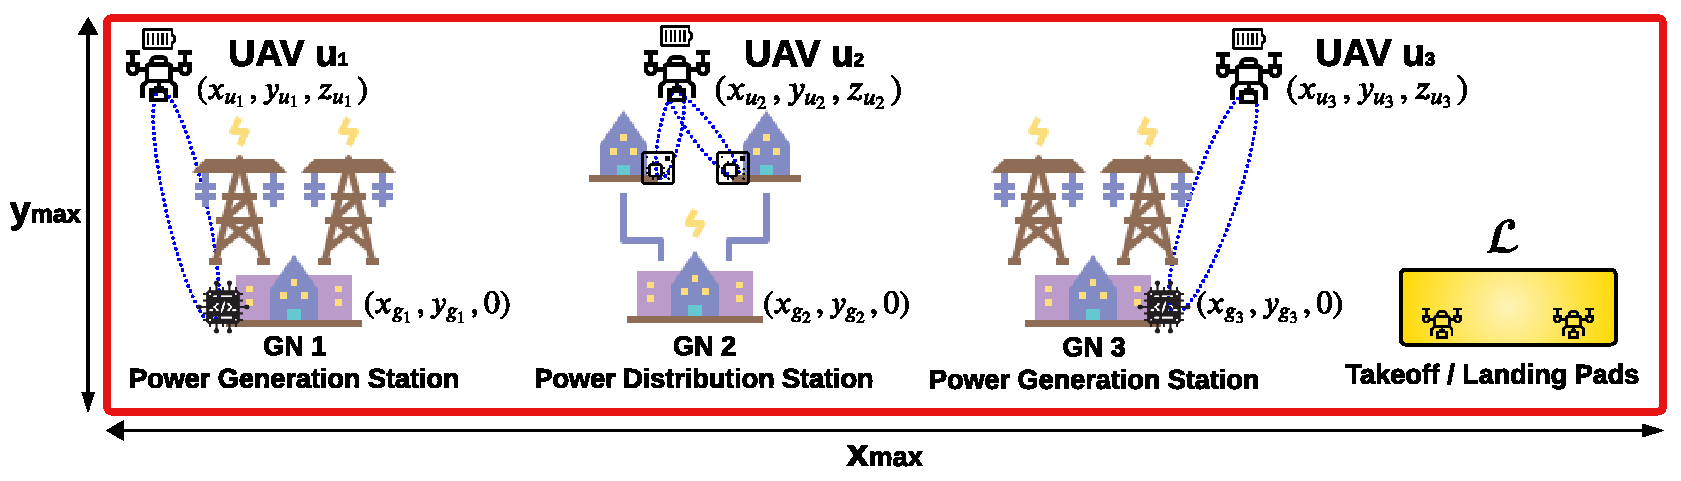
\includegraphics[width=0.8185\linewidth]{figs/deployment_model.pdf}
     \vspace{-2mm}
     \caption{Industrial automation for power grid monitoring \& restoration: Using MIMO-enabled UAVs for prioritized data harvesting from MIMO-capable GNs.}
     \vspace{-6mm}
     \label{F1}
\end{figure*}

\noindent{\textbf{Related Work}}: Several papers in the state-of-the-art detail policy frameworks to optimize the orchestration of UAVs in a variety of formulations/applications: traffic offloading and coverage extensions for terrestrial base stations using UAV relays~\cite{MAESTRO_TCCN}; maximizing the coverage area for uplink/downlink communication with ground users~\cite{Core_SoA_1_Ref_13, Core_SoA_1_Ref_14}; data harvesting from IoT devices~\cite{Core_SoA_1_Ref_12, Core_SoA_1_Ref_18_Extended_From_17, Core_SoA_1_Ref_25}; computation task offloading to UAV assisted edge networks~\cite{Core_SoA_1, Core_SoA_1_Ref_24}; capacity-maximizing distributed MIMO backhaul~\cite{CORES_ICASSP, CORES_JSAC}; and wireless power transfer~\cite{Core_SoA_1_Ref_27_Related_To_26}. While these works in the state-of-the-art tackle UAV fleet orchestration in non-terrestrial networks, they fail to address practical deployment concerns. Specifically, our prior work in this research domain~\cite{MAESTRO_TCCN} as well as the solutions in~\cite{Core_SoA_1_Ref_13, Core_SoA_1_Ref_14} fail to account for spatial multiplexing requirements, i.e., they consider single antenna UAVs and ground nodes throughout their constructions; instead, in this paper, we model the use of MIMO-enabled UAVs and MIMO-capable ground users, thereby necessitating beam-forming optimization at both ends of the communication link: precoding matrices at the ground nodes and combining matrices at the UAVs. Unlike the communication model outlined in this paper, the approaches that solve for data harvesting from MIMO-capable IoT devices using MIMO-enabled UAVs~\cite{Core_SoA_1_Ref_12, Core_SoA_1_Ref_18_Extended_From_17, Core_SoA_1_Ref_25} fail to model requests with varying degrees of priority based on their corresponding quality-of-service requirements. Contrary to the optimization formulation detailed in this work, in addition to not modeling prioritized data traffic, the works~\cite{Core_SoA_1, Core_SoA_1_Ref_24, CORES_ICASSP, CORES_JSAC, Core_SoA_1_Ref_27_Related_To_26} do not account for the on-board energy constraints of the UAVs while solving for the optimal $3$D positioning and trajectory design of the UAVs.\\
\noindent{\textbf{Novelties}}: In a nutshell, the contributions of this work can be summarized as follows. Firstly, this paper formulates the solution framework based on a system model that adequately captures the characteristics of UAV assisted wireless networks in industrial automation environments~\cite{Motivation_1, Motivation_2}: a probabilistic Air-to-Ground (A$2$G) channel model~\cite{MAESTRO_TCCN}, an uplink MIMO communication model at both the ground users as well as the UAVs, and a $3$D rotary-wing UAV mobility model (segmented $2$D with staircase transitions)~\cite{UAV_Propulsion_1} that accounts for both horizontal and vertical accelerations. Secondly, no other work in the state-of-the-art considers user requests with varying priorities and commensurate rewards: in this work, we employ a realistic quality-of-service table for various traffic flows (telemetry, file transfers, images, video streaming)~\cite{DARPA:SC2}. Thirdly, employing prioritized requests with their associated quality-of-service mandates necessitates a unique traveling salesman problem construction (with multiple UAVs) to solve for the optimal user association/scheduling mechanism (via graph-based branch-and-cut ~\cite{mTSP}). Lastly, with a constraint on the average mobility power consumption of a UAV and given its optimal $3$D position onsite, we employ a learning-based competitive swarm optimization algorithm~\cite{LCSO} to design its $3$D trajectory in a rectangular/Cartesian coordinate system.\\
\indent{The} rest of the paper is structured as: Sec.~\ref{S2} outlines the system model; Sec.~\ref{S3} elucidates our cross-layer optimization framework along with its constituent algorithms; Sec.~\ref{S4} details our numerical evaluations; Sec.~\ref{S5} lists our conclusions.
\vspace{-6mm}

%%% System model
%% Comments:
% 1. Prof. Michelusi had a comment about enforcing a distance threshold based collision avoidance mechanism among the UAVs. This is not necessary in a voxel-based design.
%    The UAVs always move/hover at the center of a voxel (e.g., <2.5, 2.5, 2.5> and <5, 2.5, 2.5>), so there's always an inherent separation between voxels.
%    Hence, at any given time, it is sufficient to enforce a voxel inequality constraint among the UAVs.
% 2. Also, on the other hand, enforcing collision avoidance this way in an offline centralized setting is nearly impossible due to the scheduling/association that is to-be-determined by mTSP.
%    So, it might be better to just say that the UAVs are equipped with LIDARs and associated sensing mechanisms (along with UAV-UAV control communication) to avoid collisions with each other (and obstacles).
%    If a UAV nears a collision while executing the LCSO optimal trajectory, it moves to the closest "collision-free" voxel.
% 3. There is an error in the description of the reward model. If the request is served sooner, since the discount factor is always less than 1, there is an additional reward.
%    The reward model can be better explained as, "The reward for serving a GN with $\delta_{\mathrm{max}}$ latency in $\delta_{gu}$ time is $\chi\gamma^{(\delta_{gu}{-}\delta_{\mathrm{max}})}$".
% 4. Additionally, as outlined earlier, the MIMO communication model needs to be explained better. The use of precoding & combining matrices can be confusing in a ZF-receiver solution.
% 5. Note that the vertical transitions model approximates the $\tilde{\kappa}$ term in the reference paper. Mention this in the description.
%    Reference: [https://ieeexplore.ieee.org/document/9461176].
% 6. Add a comment about how the comm power consumption of a rotary-wing UAV (approx. 5W) is negligible compared to its mobility power consumption (approx. 2000W).
%    So, we can safely ignore the communication power consumption characteristics of the UAV in this paper.
\section{System Model}\label{S2}
\begin{table*} [tb]
	\centering
	\begin{tabular}{|c|c|c|c|c|}
		\hline
		\textbf{Traffic Class} & \textbf{Priority} $\chi$ & \textbf{Max Latency} $\delta_{\mathrm{max}}$ mins & \textbf{Payload Size} $\nu$ Mb & \textbf{Discount Factor} $\gamma$\\
		\hline
		Telemetry & 100 & 9.1 & 256 & 0.1\\
		\hline
		File Transfer & 24 & 19.0 & 536 & 0.8\\
		\hline
		Image & 72 & 14.5 & 512 & 0.33\\
		\hline
		Video Stream & 84 & 11.6 & 1387 & 0.24\\
		\hline
	\end{tabular}
	\caption{The quality-of-service table for network flows employed in our evaluations: traffic classes, priorities, latencies, payload sizes, and discount factors~\cite{DARPA:SC2}.}
    \vspace{-6mm}
	\label{T1}
\end{table*}
\normalsize
In this section, we first outline the deployment model consisting of UAVs and ground nodes with MIMO capabilities; second, the uplink MIMO communication model at both the ground nodes as well as the UAVs; next, the probabilistic A$2$G channel model; finally, the $3$D (segmented $2$D with staircase transitions) power consumption model for rotary-wing UAVs.\\
\noindent{\textbf{Deployment Model}}: As illustrated in Fig. \ref{F1}, consider the 3D rectangular site map of a dense urban radio ecosystem of length $x_{\mathrm{max}}$, breadth $y_{\mathrm{max}}$, maximum site-wide component height of $z_{\mathrm{max}}$. This site under analysis (area $S{=}x_{\mathrm{max}}{\times}y_{\mathrm{max}}$) is tessellated into a cuboidal grid world, where each indivisible cuboid is of length $\Delta x$, breadth $\Delta y$, height $\Delta z$. With a preset mission duration of $T$, the autonomous harvesting of data from ground users is facilitated by a fleet of $U$ rotary-wing Unmanned Aerial Vehicles (UAVs), where a UAV $u \in \mathcal{U}{\triangleq}\{1,2,{\dots},U\}$ is equipped with $A_{u}$ antennas arranged in a rectangular planar array, driven by $A_{u}$ Tx/Rx chains according to a TDD protocol, for enhanced throughput and spatial multiplexing. Similarly, the $G$ Ground Nodes (GNs), scattered uniformly throughout the deployment area, possess MIMO capabilities, i.e., the communication subsystem of an aggregator/monitoring GN $g{\in}\{1,2,{\dots},G\}$ constitutes $A_{g}$ antennas arranged in a rectangular planar array (driven by $A_{g}$ Tx/Rx chains via a TDD protocol). Note that, to enforce heterogeneity in GN and UAV design, $A_{g_{1}}$ may or may not be equal to $A_{g_{2}}$, for two distinct GNs $g_{1},g_{2}$; and $A_{u_{1}}$ may or may not be equal to $A_{u_{2}}$, for two distinct UAVs $u_{1},u_{2}$. For a UAV $u{\in}\{1,2,{\dots},U\}$, let its position at the start of the mission period be denoted by $\mathbf{p}_{u}(0)$ while its position at the end of the mission period be denoted by $\mathbf{p}_{u}(T)$. Hence, $\mathbf{p}_{u}(0){\in}\mathcal{L}$ and $\mathbf{p}_{u}(T){\in}\mathcal{L}$, where $\mathcal{L}$ is the set of coordinates corresponding to the takeoff/landing pads for the UAVs: this means that the problem under consideration in this paper is an offline learning problem, solved in Sec.~\ref{S3} in a centralized fashion via a novel cross-layer optimization framework. Also, to ensure collision avoidance among the UAVs, we enforce the added condition $\mathbf{p}_{u_{1}}(t){\neq}\mathbf{p}_{u_{2}}(t),{\forall}t,{\forall}u_{1}{\neq}u_{2},u_{1},u_{2}{\in}\{1,2,{\dots},U\}$. In Sec.~\ref{S3}, this collision avoidance constraint is approached from the perspective of two UAVs not occupying the same grid voxel at the same time. With a $3$D rectangular/Cartesian coordinate system, we denote the position of UAV $u$ at time $t$ as $\mathbf{p}_{u}(t){=}(x_{u},y_{u},z_{u})$, where $0{\leq}x_{u}{\leq}x_{\mathrm{max}}$, $0{\leq}y_{u}{\leq}y_{\mathrm{max}}$, and $0{\leq}z_{u}{\leq}z_{\mathrm{max}}$. Similarly, the position of a GN $g$ is denoted by $\mathbf{p}_{g}(t){=}(x_{g},y_{g},0)$, with $0{\leq}x_{g}{\leq}x_{\mathrm{max}}$ and $0{\leq}y_{g}{\leq}y_{\mathrm{max}}$. Thus, the $3$D Euclidean distance between a GN $g$ and its serving UAV $u$ is described as $d_{gu}{=}\sqrt{(x_{u}{-}x_{g})^{2}{+}(y_{u}{-}y_{g})^{2}{+}z_{u}^{2}}$, and the elevation angle is described as $\theta_{gu}{=}\sin^{-1}{(z_{u}/d_{gu})}$.\\
\noindent{\textbf{Communication Model}}: Prior to the actual deployment of the UAV fleet, a centralized operations hub determines the subset of GNs $\mathcal{G}{\subseteq}\{1,2,{\dots},G\}$ from which the UAVs are to harvest process-critical information. In particular, an uplink transmission requirement from GN $g{\in}\mathcal{G}$ is characterized by a request header constituting its traffic class, its assigned reward/priority value $\chi$, the maximum latency $\delta_{\mathrm{max}}$ which defines its quality-of-service constraint, the size of its data payload $\nu$, and its post-deadline discount factor $\gamma$ for reward tapering. An example quality-of-service table~\cite{DARPA:SC2} for the variety of prioritized traffic flows considered in our numerical evaluations (Sec.~\ref{S4}) is shown in Table~\ref{T1}. Under this prioritized traffic model, let $\delta_{gu}$ be the time taken to harvest the data from GN $g$: if $\delta_{gu}{\leq}\delta_{\mathrm{max}}$, then the reward obtained by the UAV is $\chi$; else, the UAV gets a tapered reward $\chi \gamma^{(\delta_{gu}{-}\delta_{\mathrm{max}})}$. We operate under the assumption that a UAV in the fleet can serve multiple GNs simultaneously, but a GN can only be associated with one UAV, i.e., a GN cannot transmit its data to multiple UAVs. Additionally, once a GN is associated with a UAV, the GN fully uploads its data to the UAV (within a time duration determined by the A$2$G channel conditions as well as the beam-forming design); upon successfully offloading its data, a GN is considered to have been served. At time $t{\in}[0,T]$, let the set $\mathcal{G}_{u}{\subseteq}\mathcal{G}$ be defined as the set of GNs associated with UAV $u$. Let $\mathbf{x}_{g}{=}\boldsymbol{\Phi}_{g}{\cdot}s_{g}$ be the signal transmitted to UAV $u{\in}\{1,2,{\dots},U\}$ by GN $g{\in}\mathcal{G}_{u}$, where $\boldsymbol{\Phi}_{g}{\in}\mathbb{C}^{A_{g}{\times}1}$ denotes the linear precoding matrix used at GN $g$ and $s_{g}$ denotes the GN's message signal with $\mathbb{E}[|s_{g}|^{2}]{=}1$. If $\mathbf{H}_{gu}{\in}\mathbb{C}^{A_{u}{\times}A_{g}}$ is the channel between a GN $g{\in}\mathcal{G}_{u}$ and its serving UAV $u$, then the signal from the GN received at the UAV, i.e., $\mathbf{r}_{u}{\in}\mathbb{C}^{A_{u}{\times}1}$ is
\vspace{-0.3mm}
\begin{align}
    \mathbf{r}_{u}\ =\ \sum_{G{\in}\mathcal{G}_{u}} \boldsymbol{\Gamma}_{u}\mathbf{H}_{gu}\mathbf{x}_{g}\ +\ \mathbf{w}_{u},
\end{align}
where $\boldsymbol{\Gamma}_{u}{\in}\mathbb{C}^{A_{u}{\times}A_{u}}$ represents the combining matrix at the UAV and $\mathbf{w}_{u}{\sim}\mathcal{CN}(\mathbf{0},B_{u}N_{0}\mathbf{I}_{A_{u}})$ represents the zero-mean additive white Gaussian noise vector---with $\mathbf{w}_{u}{\in}\mathbb{C}^{A_{u}{\times}1}$, $B_{u}$ denoting the channel bandwidth allocated to UAV $u$ for its data harvesting tasks by the centralized operations hub before the start of mission execution, $N_{0}$ denoting the power spectral density of the noise, and $\mathbf{I}_{A_{u}}$ denoting the identity matrix.\\
\noindent{\textbf{A$2$G Channel Model}}: The channel between a GN $g{\in}\mathcal{G}_{u}$ and its serving UAV $u$ is described by $\mathbf{H}_{gu}{=}\sqrt{\beta}{\cdot}\boldsymbol{\Lambda}$, where $\beta$ captures the large-scale channel variations and $\boldsymbol{\Lambda}$ captures the small-scale fading effects of the channel. The large-scale effects of the communication link between the GN $g$ and its UAV $u$ can be modeled from a probabilistic LoS-NLoS view as $\beta{=}\beta_{\mathrm{LoS}}(d_{gu})\mathbb{P}_{\mathrm{LoS}}(\theta_{gu}){+}\beta_{\mathrm{NLoS}}(d_{gu})\mathbb{P}_{\mathrm{NLoS}}(\theta_{gu})$, where the LoS component $\beta_{\mathrm{LoS}}$, the NLoS component $\beta_{\mathrm{NLoS}}$, the LoS probability $\mathbb{P}_{\mathrm{LoS}}$, and the NLoS probability $\mathbb{P}_{\mathrm{NLoS}}$ terms are described as follows: $\beta_{\mathrm{LoS}}{=}\beta_{0}d_{gu}^{-\alpha}$, $\beta_{\mathrm{NLoS}}{=}\kappa\beta_{0}d_{gu}^{-\tilde{\alpha}}$, $\mathbb{P}_{\mathrm{LoS}}{=}1/(1{+}z_{1}\exp\{-z_{2}(\theta_{gu}{-}z_{1})\})$, and $\mathbb{P}_{\mathrm{NLoS}}{=}1{-}\mathbb{P}_{\mathrm{LoS}}$, with $\beta_{0}$ denoting the reference pathloss at a distance of $1$ m, $2{\leq}\alpha{\leq}\tilde{\alpha}$ denoting the pathloss exponents, $\kappa$ denoting the NLoS attenuation, and $z_{1}$ and $z_{2}$ denoting propagation parameters specific to the type of radio environment that exists at the deployment site (e.g., rural, urban, suburban). Persisting with the LoS-NLoS perspective to formulate representations for the small-scale fading effects of the channel, we model $\boldsymbol{\Lambda}$ for the LoS GN-UAV link as Rician fading with a $\theta_{gu}$-dependent $K$-factor, i.e., $K(\theta_{gu}){=}k_{1}\exp\{k_{2}\theta_{gu}\}$ (where $k_{1}$ and $k_{2}$ are propagation parameters specific to the radio environment at the deployment site); and we model $\boldsymbol{\Lambda}$ for the NLoS GN-UAV link as Rayleigh fading (i.e., Rician distribution with $K{=}0$)~\cite{MAESTRO_TCCN}.\\
\noindent{\textbf{UAV Mobility Energy Model}}: In this subsection, using the formulations in~\cite{UAV_Propulsion_1}, we discuss both the horizontal and the vertical movements of a rotary-wing UAV along with their corresponding contributions to its overall mobility energy consumption. First, under a constant horizontal velocity model, the $2$D mobility energy consumption of the UAV is given by
\vspace{-1mm}
\begin{align}\label{energy_constant_velocity}
    E_{H}(v) = \Bigg\{&P_{0}\left(1{+}\frac{3v^{2}}{u_{\mathrm{tip}}^{2}}\right) + \\&P_{1}\left(\frac{\lambda}{\omega}\right)\sqrt{\sqrt{\left(\frac{\lambda}{\omega}\right)^{2}{+}\frac{v^{4}}{4v_{0}^{4}}}{-}\frac{v^{2}}{2v_{0}^{2}}}{+}\frac{d_{0}\rho \epsilon \zeta v^{3}}{2}\Bigg\}T_{H},\nonumber
\end{align}
where $P_{j},j{=}0,1$ are scaling constants~\cite{UAV_Propulsion_1}, $v$ is the constant horizontal velocity of the UAV, $\frac{\lambda}{\omega}$ represents the UAV's thrust to weight ratio, $d_{0}$ denotes the UAV's fuselage drag ratio, $\rho$ refers to the air density, $u_{\mathrm{tip}}$ is the blade tip speed of the UAV's rotors, $v_{0}$ is the mean rotor-induced velocity of the UAV, $\epsilon$ refers to the UAV's rotor solidity factor, $\zeta$ denotes the the disc area of the UAV's rotors, and $T_{H}$ represents the duration over which the horizontal trajectory is executed~\cite{UAV_Propulsion_1}.\\
\noindent{Next}, the mobility energy consumption of the UAV under an arbitrary horizontal motion model is described as follows:
\begin{align*}
    &E_{H}(\mathbf{q}){=}\int_{0}^{T_{H}}C_{0}\left(1{+}C_{1}\Vert\mathbf{v}(\tau)\Vert^{2}\right)d\tau{+}\int_{0}^{T_{H}}C_{2}\Vert\mathbf{v}(\tau)\Vert^{3}d\tau{+}\Delta K\\&{+}\int_{0}^{T_{H}}C_{3}\sqrt{1{+}\frac{a_{\perp}^{2}(\tau)}{g^{2}}}\sqrt{\sqrt{1{+}\frac{a_{\perp}^{2}(\tau)}{g^{2}}{+}\frac{\Vert\mathbf{v}(\tau)\Vert^{4}}{C_{4}^{2}}}{-}\frac{\Vert\mathbf{v}(\tau)\Vert^{2}}{C_{4}}}d\tau,
\end{align*}
where $C_{j},j{=}0,1,{\dots},4$ are modeling parameters that depend on the UAV weight, the air density, and the UAV rotor disc area~\cite{UAV_Propulsion_1}; $\mathbf{q}$ is the arbitrary $2$D horizontal trajectory of the UAV; $\mathbf{v}(\tau){=}\dot{\mathbf{q}}(\tau)$ is the UAV's flight velocity along this trajectory; $\mathbf{a}(\tau){=}\ddot{\mathbf{q}}(\tau)$ is the UAV's horizontal acceleration along this trajectory; $a_{\perp}^{2}(\tau){=}\sqrt{\Vert\mathbf{a}(\tau)\Vert^{2}{-}\frac{(\mathbf{a}^{T}(\tau)\mathbf{v}(\tau))^{2}}{\Vert\mathbf{v}(\tau)\Vert^{2}}}$ is the UAV's centrifugal acceleration; $g$ is the acceleration due to gravity; and $\Delta K{=}\frac{1}{2}m(\Vert\mathbf{v}(T_{H})\Vert^{2}{-}\Vert\mathbf{v}(0)\Vert^{2})$ is the change in the UAV's kinetic energy~\cite{UAV_Propulsion_1}. Also, for vertical transitions, the mobility energy consumption of the rotary-wing UAV is
\vspace{0.1mm}
\begin{align*}
    &E_{V}(\mathbf{q}')\ =\ \Bigg\{\int_{0}^{T_{V}}P_{0}\left(1{+}\frac{3\Vert\mathbf{v}'(\tau){+}\mathbf{a}'(\tau)\tau\Vert^{2}}{u_{\mathrm{tip}}^{2}}\right)d\tau{+}\\&\int_{0}^{T_{V}}P_{1}\sqrt{\sqrt{1{+}\frac{\Vert\mathbf{v}'(\tau){+}\mathbf{a}'(\tau)\tau\Vert^{4}}{4v_{0}^{4}}}{-}\frac{\Vert\mathbf{v}(\tau)'{+}\mathbf{a}'(\tau)\tau\Vert^{2}}{2v_{0}^{2}}}d\tau\Bigg\}T_{V},
\end{align*}
where $P_{j},j{=}0,1$ are scaling constants~\cite{UAV_Propulsion_1}, $\mathbf{q}'$ is the arbitrary vertical trajectory of the UAV while moving to a discretized height connecting two horizontal segments, $\mathbf{v}'(\tau)$ is the initial lift velocity of the UAV along this arbitrary vertical trajectory at the start of $\tau$, $\mathbf{a}'(\tau)$ is the constant vertical acceleration of the UAV along this trajectory during $\tau$, and $T_{V}$ is the total time spent by the UAV transitioning to this different height~\cite{UAV_Propulsion_1}. Also, in the formulation detailed in Sec.~\ref{S3}, note that the UAVs are constrained in terms of their maximum flight velocity ($v_{\mathrm{max}}$) and their maximum acceleration ($a_{\mathrm{max}}$), in both the horizontal and vertical directions. Finally, given these energy consumption models of the rotary-wing UAV for horizontal and vertical trajectories, we can construct the complete $3$D energy consumption model of a UAV $u{\in}\{1,2,{\dots},U\}$ as $E_{u}(\mathcal{Q},\mathcal{Q}'){=}\sum_{\mathbf{q}{\in}\mathcal{Q}}E_{H}(\mathbf{q}){+}\sum_{\mathbf{q}'{\in}\mathcal{Q}'}E_{V}(\mathbf{q}')$, where $\mathcal{Q}$ is the set of horizontal trajectory segments in the overall optimal $3$D trajectory of the UAV (obtained via learning-based competitive swarm optimization in Sec.~\ref{S3}), while $\mathcal{Q}'$ is the set of segments representing the vertical transitions between two horizontal segments from $\mathcal{Q}$. While communicating with the GNs in $\mathcal{G}_{u}$, the UAV hovers at the corresponding optimal position until it fully receives the uplink data transmissions from all GNs $g{\in}\mathcal{G}_{u}$: here, the energy consumption of the UAV is obtained from \eqref{energy_constant_velocity} as $E_{S}(0){=}1376{\cdot}T_{S}$ Joules~\cite{UAV_Propulsion_1}, where $T_{S}$ is the time taken by the UAV to harvest data from its associated users.
\vspace{-6mm}

%%% Cross-layer optimization: The radio and vehicle layers
%% Comments:
% 1. As outlined earlier, the collision avoidance constraint is hard to implement in a offline centralized setting and may not be needed.
% 2. Re-write the "precoding & combining matrices" solution variables description as "beam-forming design". Also, rename the "branch-and-cut" method as "branch-and-bound".
%    Cite the Gavish and Srikanth paper whenever you mention "branch-and-bound". Furthermore, as mentioned earlier, refer to the LCSO algorithm as "Learning Competitive Swarm Optimization".
% 3. The ZF description in the "fine-search" sub-section is better described as follows:
%    "...using ZF receivers at the UAV to perform channel inversion, extract the desired symbols, evaluate the resultant SINR, determine the resultant channel capacity, and thus obtain the GN service latency..."
% 4. Also, I think we need to flip the solution sequence order: LCSO gives us the trajectories (and their costs) of the edges between nodes; then, mTSP branch-and-bound solves for the scheduling/association.
% 5. Additionally, the descriptions of the forward, intermediate, and return trajectories have to be updated because the mTSP-LCSO solution order has been flipped. LCSO designs all trajectories before mTSP uses these traj costs.
% 6. Lastly, the "generalization mapping" in the LCSO subsection from (p, v, \upsilon, \eta) to (\psi, \xi) is not very clear. Rewrite this description.
\section{Cross-Layer Optimization Formulation}\label{S3}
The overall objective of the solution framework proposed in this paper is to maximize the fleet-wide reward obtained by successfully harvesting prioritized data traffic from the GNs onsite over a preset finite mission execution time. Specifically,
\begin{align}\label{Opt}
    &\max_{\mathcal{S}}\ \sum_{t=1}^{T}\ \sum_{u \in \mathcal{U}}\ \sum_{g \in \mathcal{G}_{u}}\chi_{g}\gamma^{(\delta_{gu} - \delta_{\mathrm{max}})} \text{ s.t. }\\
    &\mathbf{p}_{u}(0) \in \mathcal{L}, \mathbf{p}_{u}(T) \in \mathcal{L}, \forall u \in \mathcal{U},\label{C1}\tag{C.1}\\
    &\mathbf{p}_{u_{1}}(t) \neq \mathbf{p}_{u_{2}}(t), \forall u_{1}, u_{2} \in \mathcal{U}, u_{1} \neq u_{2}, \forall t,\label{C2}\tag{C.2}\\
    &g \in \mathcal{G}_{u_{1}}{\implies}g \notin \mathcal{G}_{u_{2}}, u_{1}, u_{2} \in \mathcal{U}, u_{1} \neq u_{2}, g \in \mathcal{G},\label{C3}\tag{C.3}\\
    &P_{u}(t) \leq P_{\mathrm{avg}}, v_{u}(t) \leq v_{\mathrm{max}}, a_{u}(t) \leq a_{\mathrm{max}}, \forall u \in \mathcal{U},\label{C4}\tag{C.4}
\end{align}
where $\mathcal{S}$ represents the set of optimization variables, i.e., the GN association/scheduling mechanism, the precoding and combining matrices constituting the beam-forming design, the $3$D positions of the UAVs to serve their respective scheduled GNs, and the $3$D energy-conscious forward, intermediate, and return trajectories of the UAVs. The constraints defining this optimization problem include the UAV start- and end-position enforcement in \eqref{C1}; the UAV collision avoidance in \eqref{C2}; the GN-UAV scheduling exclusivity in \eqref{C3}; and the UAV average mobility power consumption, the UAV maximum velocity, and the UAV maximum acceleration in \eqref{C4}. Given the complexity of this optimization problem, we decompose it into inter-connected radio and vehicle layer sub-problems and solve each problem separately (via its corresponding proposed algorithm). First, we simplify the GN association/scheduling strategy by clustering the GNs according to their proximity in deployment onsite; then, with zero-forcing beam-forming, we employ a coarse- and a fine-grained exhaustive search to find the optimal $3$D voxel in the grid for UAV positioning; next, we employ a multiple traveling salesman problem formulation and solve it using a graph-based branch-and-cut technique to obtain the optimal GN association/scheduling mechanism; finally, the learning-based competitive swarm optimization algorithm is used to design the optimal $3$D UAV trajectories.\\
\noindent{\textbf{K-Means GN Clustering}}: To solve for the optimal $3$D UAV positioning and the subsequent GN association/scheduling strategy, we first group the GNs in the network into $C{\leq}U$ clusters according to their onsite deployment proximity. In this regard, we employ the K-means clustering algorithm to minimize the intra-cluster sum-of-squares cost function, i.e., to obtain the set of GN clusters $\{\mathcal{G}_{1},\mathcal{G}_{2},{\dots},\mathcal{G}_{C}\}$, the standard K-means algorithm is used to solve the following problem:
\begin{align}\label{Clustering}
    &\argmin_{\{\mathcal{G}_{1},\mathcal{G}_{2},{\dots},\mathcal{G}_{C}\}} \sum_{c = 1}^{C} \sum_{\mathbf{p} \in \mathcal{G}_{c}} ||\mathbf{p} - \boldsymbol{\mu}_{c}||^{2}\ \text{s.t.}\\
    &C \leq U \text { and } |\mathcal{G}_{1}| + |\mathcal{G}_{2}| + \dots + |\mathcal{G}_{C}| = |\mathcal{G}|.\nonumber
\end{align}
Here, $\boldsymbol{\mu}_{c}$ is the centroid (or mean) of the GNs in a cluster $\mathcal{G}_{c}, c{\in}\{1,2,{\dots},C\}$, i.e., $\boldsymbol{\mu}_{c}{=}\frac{1}{|\mathcal{G}_{c}|}\sum_{\mathbf{p}{\in}\mathcal{G}_{c}}\mathbf{p}$. This algorithm is a generalized variant of the Expectation-Maximization (EM) algorithm, wherein with the Forgy method of initializing the cluster centroids, the expectation step (E-step) involves assigning each GN to the cluster with the nearest centroid (least squared Euclidean distance) while the maximization step (M-step) involves recalculating the centroids for each cluster; this iterative back-and-forth between the E-step and the M-step continues until the GN cluster assignments no longer change.\\
\noindent{\textbf{Grid Search for UAV Positioning}}: Upon clustering the GNs onsite, we employ a dual-stage grid search technique to determine the optimal $3$D positioning of a UAV serving each of these clusters. The first-stage of this positioning scheme involves a bounding-box strategy to determine the larger set of $3$D grid voxels: specifically, all the voxels within the smallest area subset encapsulating all GNs in a cluster constitutes the argument set for the finer-grained exhaustive grid search in the second-stage. In the second-stage, with a Zero-Forcing (ZF) beam-forming technique to design the precoding (at the GNs) and combining matrices (at the UAV), we evaluate the cluster-wide reward at each voxel; then, we pick the voxel that maximizes this reward as the optimal serving UAV position.\\
\noindent{\textbf{UAV-GN Scheduling via mTSP}}: Next, to solve for the optimal GN association/scheduling strategy, we formulate a multiple Traveling Salesman Problem (mTSP) setup~\cite{mTSP}, wherein with the added constraints of having to start and end at a root node (landing pads), the inherent objective is to plan the routes of the UAVs in the network (i.e., salesmen) to serve the GN clusters onsite (at the corresponding $3$D voxels obtained earlier via dual-stage grid search) while minimizing the value of the cost function (determined by the quality-of-service experienced by the GNs) imposed within this construction. Overlaying a fully-connected graph on this deployment, the vertices of the consequent graph are the optimal positions of serving UAVs (per cluster) while the edges of the graph include the lines connecting said vertices; this novel mTSP approach is solved via a branch-and-cut method~\cite{mTSP} to obtain the association of UAVs in the fleet with specific GN clusters as well as the scheduling sequence in which a particular UAV goes about serving its associated clusters. After obtaining the optimal user association/scheduling mechanism, knowing the optimal positions of the serving UAVs per cluster, via the learning competitive swarm optimization algorithm, we design the forward, intermediate, and return trajectories of the UAVs.\\
\noindent{\textbf{UAV Trajectory Design via LCSO}}: Given the initial position of a UAV $u$, i.e., $\mathbf{p}_{u}(0){\in}\mathcal{L}$, and its optimal serving position(s) $\{\mathbf{p}_{u,1},\mathbf{p}_{u,2},{\dots}\}$ to harvest data from its assigned cluster(s) of GNs $\{\mathcal{G}_{u,1},\mathcal{G}_{u,2},{\dots}\}$, we use the learning competitive swarm optimization algorithm to design the forward, intermediate, and return trajectories of the UAV. Under a \emph{stop-and-receive} protocol and given the GN association/scheduling strategy determined via our aforementioned mTSP formulation, the UAV's forward trajectory $\mathbf{q}_{u}$ involves the set of way-points and velocities from its starting position $\mathbf{p}_{u}(0)$ to the optimal serving position for its first GN cluster $\mathcal{G}_{u,1}$; then, upon successfully harvesting data from all the active GNs in this cluster, the UAV possesses multiple intermediate trajectories from the optimal position of its previously scheduled GN cluster (e.g., $\mathcal{G}_{u,1}$) to the optimal position of its next scheduled GN cluster $\mathcal{G}_{u,2}$; finally, the return trajectory constitutes the set of way-points and velocities from the optimal position for its final GN cluster to a landing position $\mathbf{p}_{u}(T){\in}\mathcal{L}$. The Learning Competitive Swarm Optimization (LCSO) algorithm~\cite{LCSO} is a highly-scalable and a computationally efficient variant of the popular Competitive Swarm Optimization (CSO) algorithm typically used for route planning~\cite{MAESTRO_TCCN}, thereby making it a suitable candidate for energy-conscious $3$D UAV trajectory design. LCSO constitutes a dual-stage process: formulating sub-swarms in the swarm of particles (i.e., UAV way-points and velocities), the algorithm's first-stage involves organizing tournaments within the sub-swarms while the second-stage involves tournaments among these sub-swarms. In particular, first, the randomly initialized swarm of $N_{S}$ particles $(\mathbf{p}, v)_{1:N_{S}}$ and their associated particle velocities $(\boldsymbol{\upsilon}, \eta)_{(1:N_{S})}$ is grouped into $N_{SS}$ sub-swarms; then, in each iteration $i$, every particle $(\mathbf{p}, v)$ in a sub-swarm competes in a tournament with the other particles in the sub-swarm as follows based on an evaluation objective determined by the $3$D mobility energy consumption of the UAV (see Sec.~\ref{S2}). These tournaments are organized independently and in parallel across all the sub-swarms. Specifically, each such tournament within an individual sub-swarm involves the following procedure: first, randomly select three particles; next, compute and compare their evaluation objective; consequently, determine a winner $\boldsymbol{\psi}_{w}$, a runner-up $\boldsymbol{\psi}_{r}$, and a loser $\boldsymbol{\psi}_{l}$; subsequently, modify the knowledge of the runner-up and the loser particles based on the attributes of the winner according to the following equations:
\begin{align}\label{LCSO_1}
    &\boldsymbol{\xi}_{r}(i + 1) = n_{1}\boldsymbol{\xi}_{r}(i) + n_{2}\left(\boldsymbol{\psi}_{w}(i) - \boldsymbol{\psi}_{r}(i)\right);\nonumber\\
    &\boldsymbol{\psi}_{r}(i + 1) = \boldsymbol{\psi}_{r}(i) + \boldsymbol{\xi}_{r}(i + 1);\nonumber\\
    &\boldsymbol{\xi}_{l}(i{+}1){=}n_{1}\boldsymbol{\xi}_{l}(i){+}n_{2}\left(\boldsymbol{\psi}_{w}(i){-}\boldsymbol{\psi}_{l}(i)\right){+}n_{3}\left(\boldsymbol{\psi}_{r}(i){-}\boldsymbol{\psi}_{l}(i)\right);\nonumber\\
    &\boldsymbol{\psi}_{l}(i + 1) = \boldsymbol{\psi}_{l}(i) + \boldsymbol{\xi}_{l}(i + 1);
\end{align}
where $\boldsymbol{\xi}_{w}$, $\boldsymbol{\xi}_{r}$, and $\boldsymbol{\xi}_{l}$ correspond to the particle velocities of the winner, runner-up, and loser particles, respectively; and $n_{1}$, $n_{2}$, and $n_{3}$ are uniformly generated random numbers in the range $[0,1]$. Next, the second stage of the LCSO algorithm constitutes a tournament among the sub-swarms: randomly choose a particle from among the winners of each sub-swarm; then, randomly choose three particles from this set of winners; after which, compute and compare their evaluation objectives to determine a winner $\boldsymbol{\psi}_{w}$, a runner-up $\boldsymbol{\psi}_{r}$, and a loser $\boldsymbol{\psi}_{l}$; next, update the knowledge of the runner-up and the loser particles based on the attributes of the winner according to the set of equations detailed in~\eqref{LCSO_1}. This iterative two-stage process of the LCSO algorithm continues until the total number of constituent computations of the underlying objective function (UAV energy consumption) exceeds a preset threshold~\cite{LCSO}.\\
\indent{In} summary, the optimal orchestration of a fleet of MIMO UAVs harvesting prioritized data traffic from MIMO-enabled GNs involves the following algorithmic process: first, we cluster the GNs using the naive K-means clustering algorithm; then, employing a coarse- (cluster bounding-box candidates) and a fine-grained (multi-user MIMO ZF beam-forming to compute service latencies) reward-maximizing exhaustive grid search, we obtain the cluster-wise optimal serving positions; next, we employ the graph-based branch-and-cut technique to solve for the optimal cluster association/scheduling strategy formulated as an mTSP; and finally, knowing the schedules and the optimal serving positions for the UAVs, we utilize the LCSO mechanism (with a UAV mobility energy consumption cost function) to design the energy-optimal $3$D trajectories.
\vspace{-6mm}

%%% Numerical evaluations
%% Comments:
% 1. Double-check the simulation parameters before the camera-ready copy is due. I have a feeling that the channel parameters may have been modified.
% 2. The SU-MIMO evaluation of IGD and IBF has been modified. Change the descriptions accordingly.
%    IGD & IBF: Determine the optimal Rx ANT positions in a distributed MIMO setup to serve each GN in a UAV's designated cluster.
%               Then, a distance minimization heuristic determines the cluster-wide optimal serving position of the UAV. The distributed Rx ANT positioning mechanism is adapted from the IGD/IBF impl in Hanna et al.
% 3. Moreover, do not refer to the X-axis in Fig. 2 as a constraint. It is not necessarily equal to the P_avg constraint imposed in LCSO. It's the average per-UAV mobility power consumption evaluated at the end of the mission.
\section{Numerical Evaluations}\label{S4}
In this section, we describe the numerical evaluations underlying our research efforts in order to demonstrate the functionalities and performance characteristics of the proposed cross-layer optimization framework to orchestrate a fleet of energy-conscious UAVs for MIMO-enabled prioritized data harvesting. First, we outline our simulation setup; next, we detail our evaluation criteria; finally, we compare and contrast the attributes of our solution against static UAV deployment heuristics as well as the iterative gradient descent and the iterative brute force algorithms from the state-of-the-art~\cite{CORES_ICASSP}.\\
\noindent{\textbf{Simulation Setup}}: In this work, we simulate a fleet of $U{=}6$ rotary-wing UAVs ($A_{u}{=}16,{\forall}u{\in}\{1,2,{\dots},U\}$) serving a set of $G{=}36$ randomly distributed heterogeneous GNs ($A_{g}{=}4,{\forall}g{\in}\{1,2,{\dots},G\}$) deployed across a cuboidal grid world with dimensions $x_{\mathrm{max}}{=}5$ km, $y_{\mathrm{max}}{=}5$ km, $z_{\mathrm{max}}{=}0.2$ km, $\Delta x{=}5$ m, $\Delta y{=}5$ m, and $\Delta z{=}5$ m. Using the K-means clustering algorithm detailed earlier, we cluster the GNs into a maximum of $C{=}6$ clusters, each containing at least one GN. The bandwidth of each data channel is $5$ MHz (each UAV is pre-assigned a data channel to service its GNs), the LoS pathloss exponent $\alpha$ is $2$, the NLoS pathloss exponent $\tilde{\alpha}$ is $2.8$, the NLoS attenuation constant $\kappa$ is $0.2$, and the SNR referenced at a distance of $1$ m is $40$ dB. Additionally, the Rician K-factor parameters are $k_{1}{=}1$ and $k_{2}{=}0.05$, while the LoS probability parameters are $z_{1}{=}9.61$ and $z_{2}{=}0.16$. Lastly, the mobility parameters of the rotary-wing UAV are obtained from~\cite{UAV_Propulsion_1}, with added constraints $v_{\mathrm{max}}{=}55$ m/s, $a_{\mathrm{max}}{=}5$ m/$\text{s}^{2}$.\\
\begin{figure*}[t]
    \centering
    \begin{subfigure}{0.4925\linewidth}
        \centering
        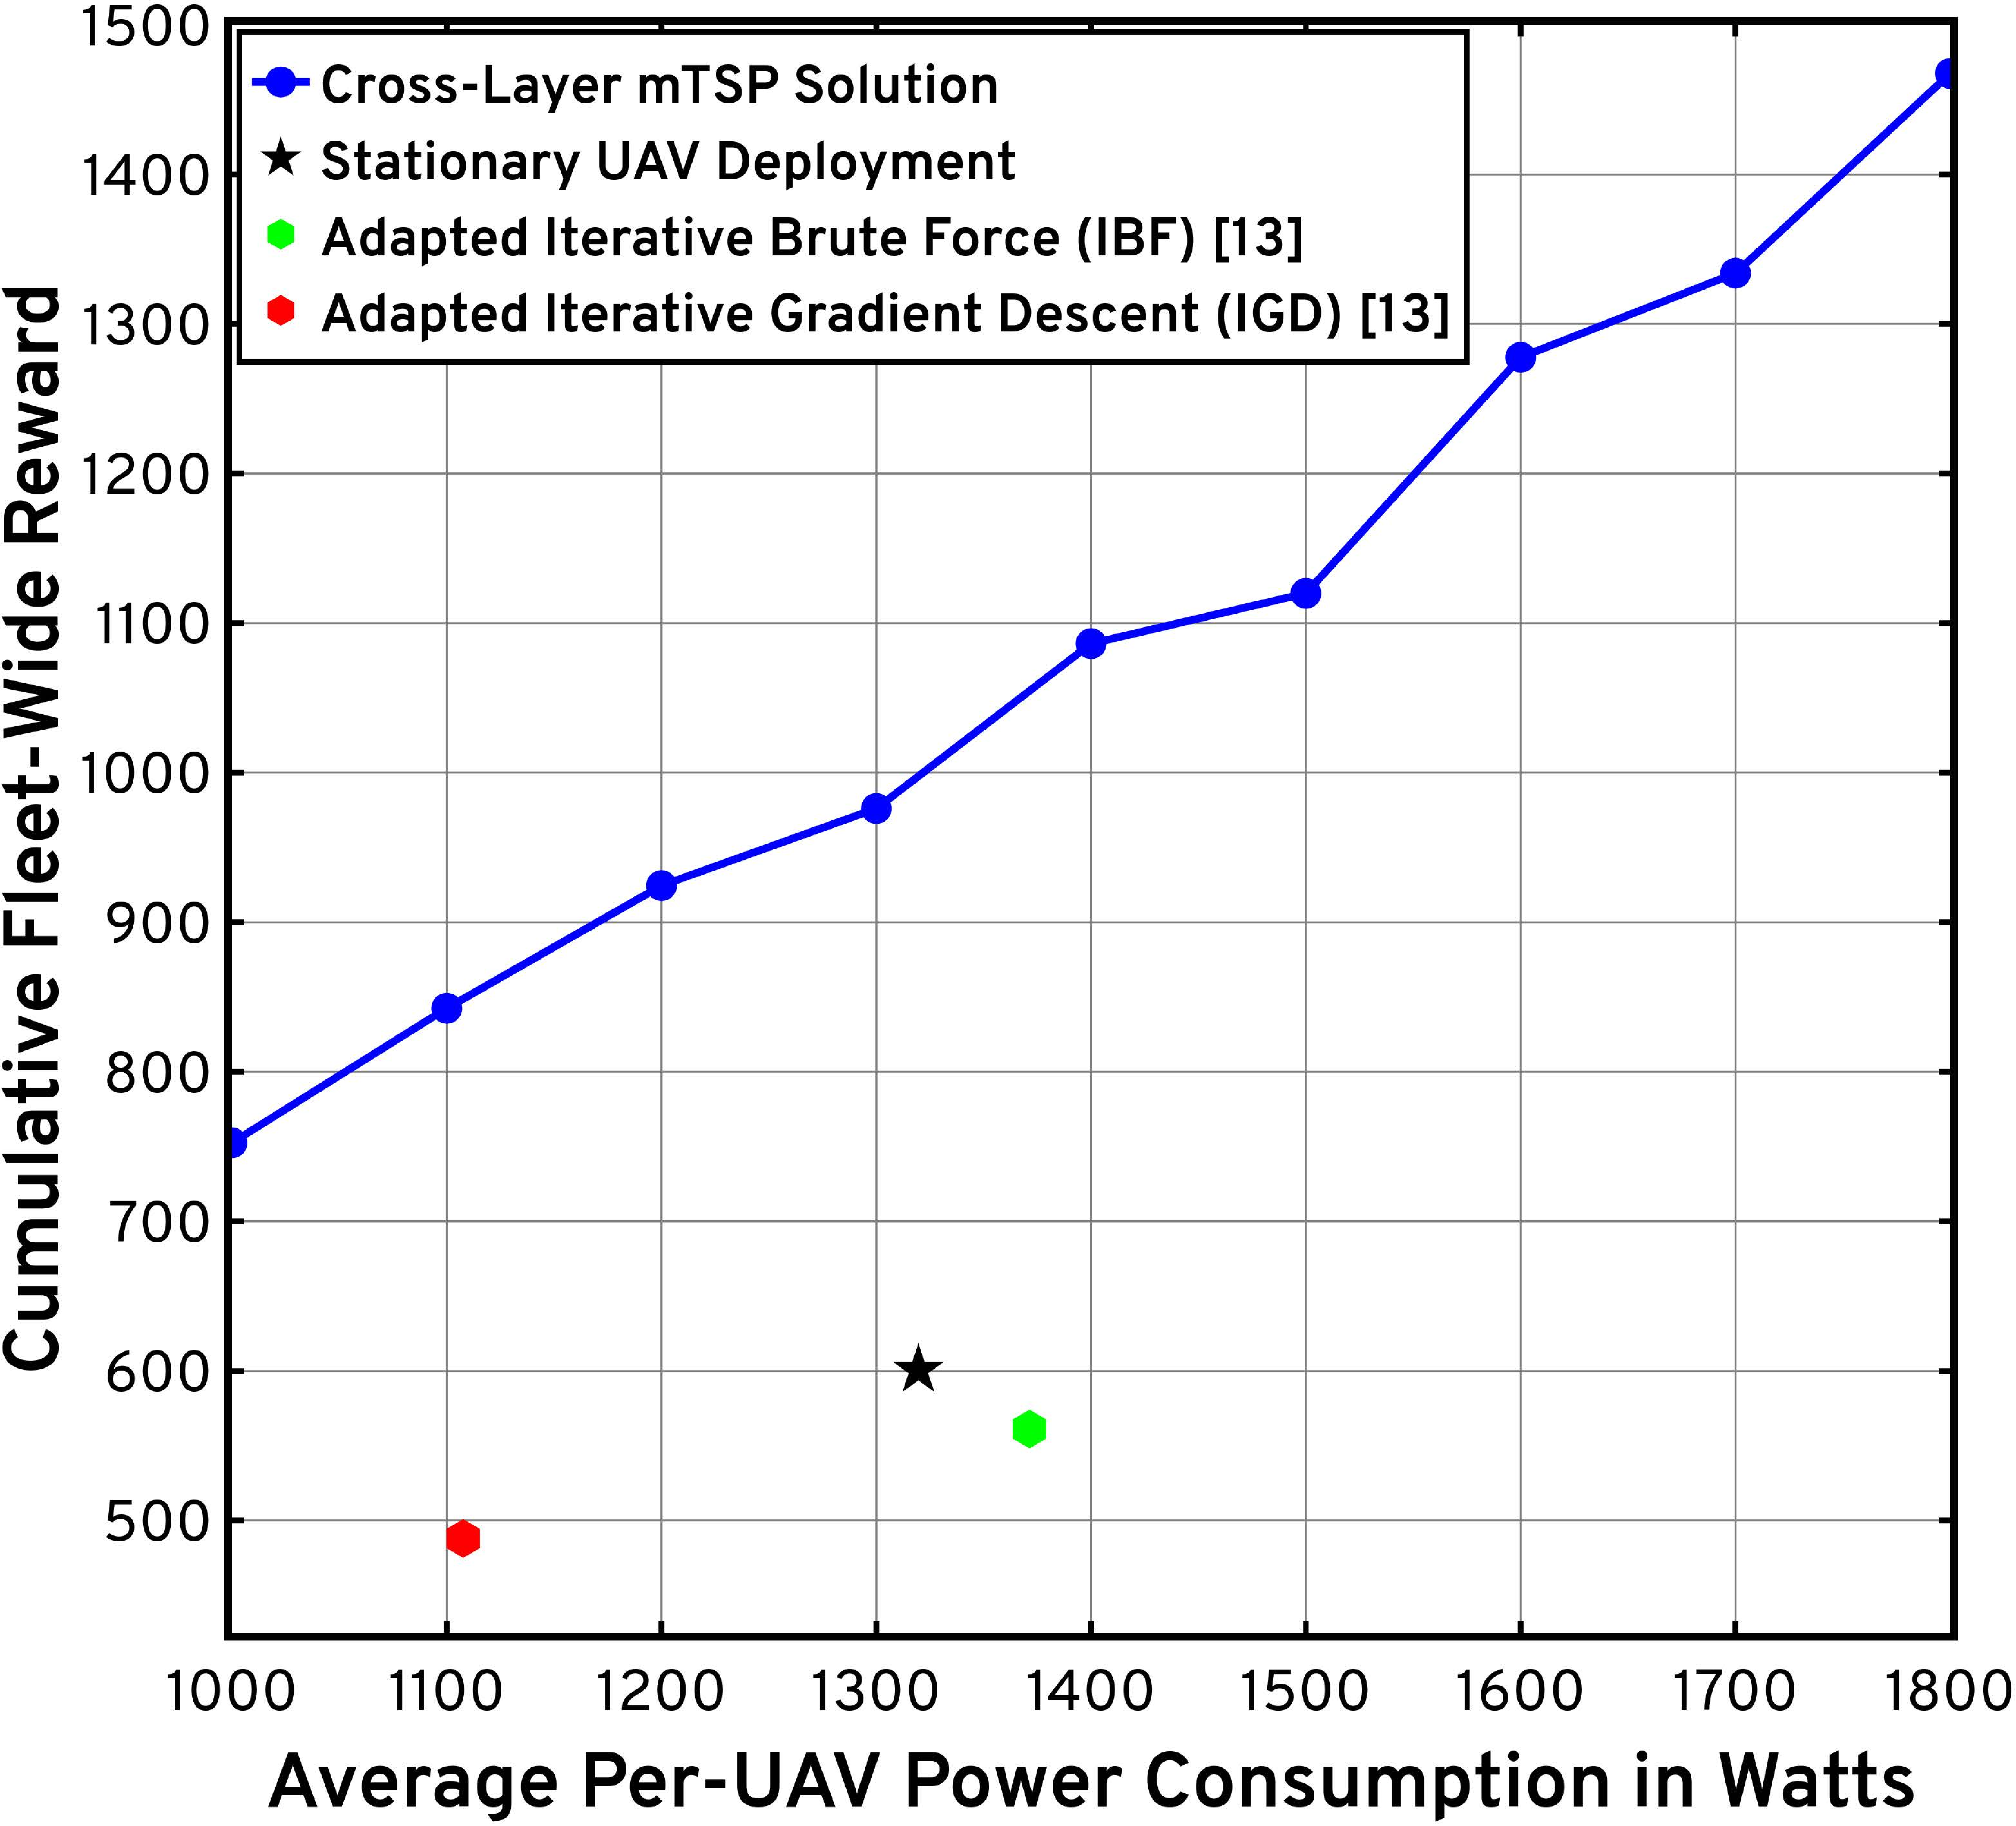
\includegraphics[width=0.81\linewidth]{figs/reward_vs_average_power.pdf}
        \vspace{-1mm}
        \caption{Cumulative Fleet-Wide Reward vs Average Per-UAV Power Consumption}
        \label{F2a}
    \end{subfigure}
    \begin{subfigure}{0.4975\linewidth}
        \centering
        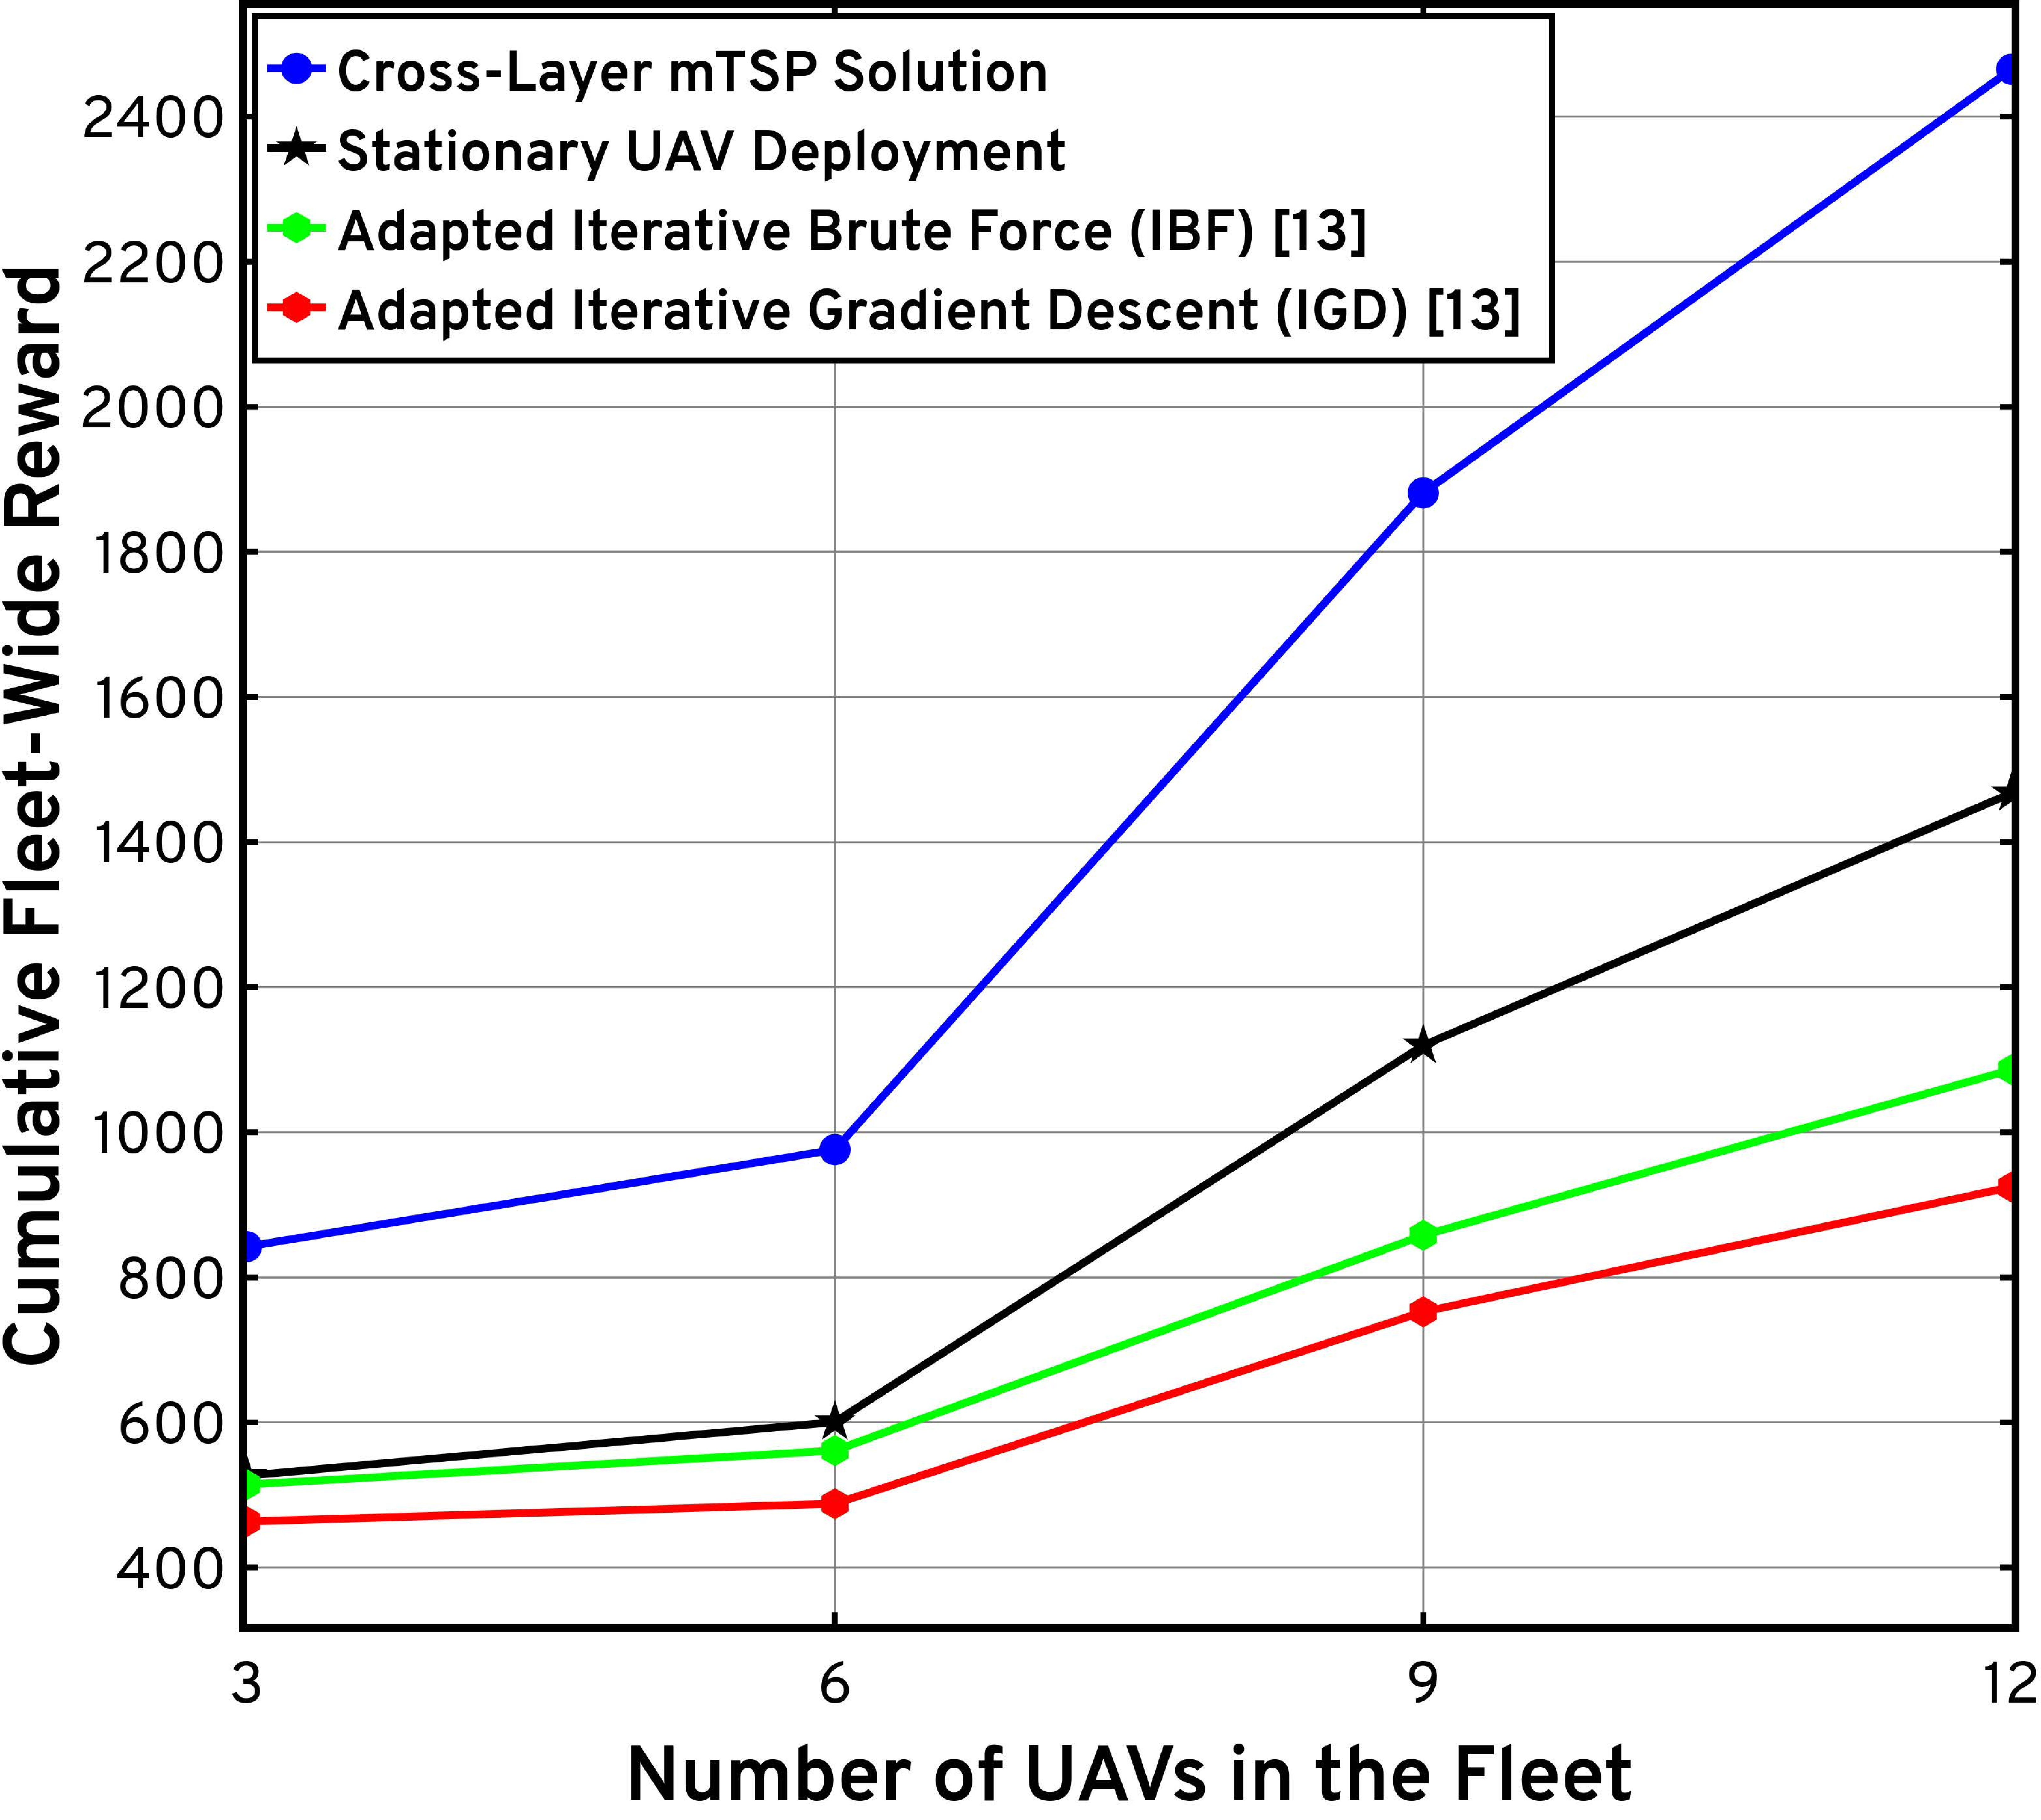
\includegraphics[width=0.81\linewidth]{figs/reward_vs_number_of_uavs.pdf}
        \vspace{-1mm}
        \caption{Cumulative Fleet-Wide Reward vs Number of UAVs in the Fleet}
        \label{F2b}
    \end{subfigure}
    \vspace{-6mm}
    \caption{A plot depicting the total reward accumulated by the UAVs in the fleet over the mission simulation period vs average per-UAV power consumption (a); and a plot depicting the total reward vs number of UAVs in the fleet (b). The plots also show evaluations against the state-of-the-art (static, IGD \& IBF~\cite{CORES_ICASSP}).}
    \vspace{-6mm}
    \label{F2}
\end{figure*}
\indent{With} the simulation setup described earlier, we evaluate the performance of the cross-layer optimization solution proposed in this paper with stationary UAV deployment heuristics and relevant schemes adapted from the current literature~\cite{CORES_ICASSP}. For the stationary deployment scheme, coupled with the K-means clustering strategy (with fixed $C{=}U{=}6$) and a multi-user MIMO ZF beam-forming design, we statically position each of the $6$ UAVs at the centroid of their respective cluster and evaluate the fleet-wide reward obtained over the preset mission duration. On the other hand, for the Iterative Gradient Descent (IGD) and the Iterative Brute Force (IBF) algorithms adapted from~\cite{CORES_ICASSP} to suit our network modeling, upon clustering the GNs (with fixed $C{=}U{=}6$), each UAV in its pre-assigned cluster serves each constituent GN in a sequential manner (ranked in increasing order of maximum allowed latency), with the optimal UAV position obtained via the IGD and IBF algorithms~\cite{CORES_ICASSP} and single-user MIMO ZF beam-forming dictating the communication characteristics underlying the evaluation objective. Thus, Fig.~\ref{F2a} depicts the total reward accumulated by the fleet using our solution as a function of the average per-UAV power consumption constraint ($P_{\mathrm{avg}}$) over the simulated mission duration ($T{=}1800$ s). Note that, for stationary deployment heuristic as well as for the IGD and IBF algorithms, to ensure fairer comparisons with the our solution, we account for the transitions of the UAVs to-and-from the takeoff/landing pads by incorporating the corresponding movement delays (\emph{as the crow flies} with a constant velocity of $v_{\mathrm{max}}$ at a fixed height of $200$ m). For similar power levels, we demonstrate a $58$\% gain over stationary deployments, a $70$\% gain over the IGD scheme from~\cite{CORES_ICASSP}, and a $78$\% gain over the IBF scheme from~\cite{CORES_ICASSP}. Next, Fig.~\ref{F2b} illustrates the cumulative fleet-wide reward as a function of the number of UAVs $U$ in the fleet (fixed $G{=}36$) along with the reference benchmarks of a stationary UAV deployment as well as the IGD and IBF schemes from~\cite{CORES_ICASSP}: here, we show that, as expected, the reward accumulated by the fleet increases with the number of UAVs; and that our proposed cross-layer mTSP solution consistently (across $3$, $6$, $9$, and $12$ UAVs) out-performs both the stationary deployments as well as the IGD and IBF schemes from~\cite{CORES_ICASSP}.
\vspace{-3mm}

%%% Concluding remarks and Future work
%% Comments: 
% 1. As mentioned earlier, refer to the "branch-and-cut" method as the "branch-and-bound" method.
% 2. Also, I think we need to flip the solution sequence order: LCSO gives us the trajectories (and their costs) of the edges between nodes; then, mTSP branch-and-bound solves for the scheduling/association.
\section{Conclusion}\label{S5}
In this work, we describe the orchestration of a fleet of energy-conscious MIMO-enabled rotary-wing UAVs for harvesting prioritized data traffic from a random distribution of heterogeneous MIMO-capable GNs. With a preset mission duration and grid-world tessellation, the fleet-wide reward maximization problem is solved offline under a cross-layer optimization construction. Upon clustering the ground nodes via K-means clustering, we first employ a grid-bounding technique to determine the set of candidate $3$D voxels for UAV positioning; then, employing a ZF beam-forming design, we determine the optimal latency-minimizing $3$D voxel among this set of candidate voxels; next, via a branch-and-cut method to solve the underlying mTSP, we obtain the optimal GN association/scheduling mechanism; consequently, we solve for the optimal $3$D trajectories of the UAVs via LCSO. Numerical evaluations illustrate that our solution outperforms static UAV deployments as well as state-of-the-art IGD and IBF schemes vis-\'{a}-vis GN quality-of-service and UAV energy efficiency.
\vspace{-3mm}

% References (main.bib)
\bibliographystyle{IEEEtran}
\bibliography{IEEEabrv,main}

\end{document}
% Content ends